\documentclass[10pt]{article}
\usepackage{icmlko}

\icmlmeta{IP 파운데이션 월드모델}{35}{결측이 라벨을 알고 있었다}{배선을 검정으로 고르는 도구를 만들었더니 그 도구가 바로 앞 노트를 무너뜨렸다 --- 도서의 자기 상관은 판형이 아니라 매체 형식이었다}

\begin{document}

\twocolumn[
\icmlheader

\begin{abstract}
노트 34는 배선이 유일하게 남은 지렛대라고 결론지었다. 그래서 배선을 의미가
아니라 검정으로 고르는 탐색기를 만들었다. 도메인마다 관측 가능한 원변수를 전부
모아 축 슬롯별로 무엇이 가장 강한지 잰다. 두 가지가 나왔다. 첫째, 게임에서
\textbf{내가 꺼 놓은 두 축이 라벨과 가장 강하게 상관}한다(가격 $+$0.351,
퍼블리셔 이력 $+$0.280). 둘째, 도서의 굿즈 규모에 넣은 쪽수($-$0.015)보다
\textbf{양장 여부($+$0.296)}가 훨씬 강하다. 그런데 둘을 실제로 갈아 끼우자
결과가 갈렸다 --- 꺼진 축을 켜면 유의 방향이 9에서 \textbf{7로 떨어지고}, 슬롯
안에서 변수만 바꾸면 9에서 \textbf{11로 오른다}. 축을 켜는 것은 공통 축 집합과
정렬 기하를 바꾸므로 단독 상관으로 판단할 수 없다. 여기까지가 계획한 일이고,
확인하다가 훨씬 나쁜 것이 나왔다. 도서의 판형은 61\%만 관측되는데 \textbf{관측
안 되는 154건이 전부 전자책}이고, 두 형식의 판매지수는 log 평균 4.30 대 3.31로
\textbf{열 배} 차이 난다. 즉 판형을 쓰는 축은 물리량을 재는 척하면서 매체 형식을
맞힌다. 형식별 평균을 빼자 도서 자기 상관이 \textbf{0.459에서 $-$0.002로
사라졌다}. 노트 34의 ``판형으로 배선하니 3.4배''는 이 누출을 포함한 값이다.
전자책을 빼고 243건으로 다시 세우니 자기 상관은 0.203으로 낮아졌지만, 도서를
출처로 쓴 세 방향이 \emph{모두 좋아졌고}(→팝업 $-$0.070$\to-$0.079,
→아이돌 $-$0.040$\to-$0.064) 노트 33의 등식은 $+$0.930에서
\textbf{$+$0.983으로 오히려 깨끗해졌다}.
\end{abstract}
]

\section{배선을 검정으로 고르는 도구}

노트 34의 결론은 ``전이 성능은 배선으로 바꿀 수 있고 그것이 유일하게 남은
지렛대다''였다. 같은 노트에 실수를 세 번 반복했다는 기록도 남겼다 --- 노트 25,
28, 그리고 34. 매번 \emph{의미로는 맞아 보이는} 배선이었다.

그래서 규칙을 코드로 만들었다. 도메인마다 관측 가능한 원변수를 전부 모아 각 축
슬롯에 무엇을 넣을지 검정으로 고른다. 두 제약을 건다 --- 라벨을 쓰지 않는 변수만
후보로 두고, 축마다 허용 유형을 선언해 도메인 간 기능 정합을 강제한다(노트 20·23).

\paragraph{첫 실행이 부호를 뒤집었다}
처음에는 0의 비율로 ``이 0이 결측인가 정상값인가''를 추측하게 했다. 그러면 이진
변수(0/1)와 결측(0)이 섞인다. 도서 판형은 61\%만 관측되는데 나머지 39\%의
`높이 0'이 상관에 들어가 부호가 뒤집혔다 --- 노트 34에서 $-$0.282였던 것이
$+$0.712로 나왔다. 결측은 호출부에서 명시하도록 고쳤다. \emph{이 오류가 뒤에
나올 진짜 문제의 첫 신호였다는 것은 그때 몰랐다.}

\begin{table}[t]
\centering\tsize
\caption{슬롯별 최선 변수(결측 명시 후).}
\begin{tabular}{llrr}
\toprule
도메인 & 변수 & 슬롯 & 라벨과 r \\
\midrule
게임 & 설치 용량 & 굿즈 규모 & $+$0.416 \\
게임 & \textbf{가격} & \textbf{입장 허들} & $+$0.351 \\
게임 & \textbf{퍼블리셔 이력} & \textbf{매장 노출도} & $+$0.280 \\
게임 & 지원 언어 수 & 타깃 폭 & $+$0.176 \\
\midrule
도서 & \textbf{양장 여부} & \textbf{굿즈 규모} & $+$0.296 \\
도서 & 판형 높이(역) & 타깃 폭 & $+$0.283 \\
도서 & 정가 & 입장 허들 & $+$0.205 \\
도서 & 쪽수 & 굿즈 규모 & $-$0.015 \\
\midrule
아이돌 & 소속사 사전 데뷔 & 매장 노출도 & $+$0.345 \\
아이돌 & 인원 수 & 타깃 폭 & $+$0.234 \\
\bottomrule
\end{tabular}
\end{table}

굵은 것이 현재 배선과 다른 셋이다. 게임의 두 축은 \textbf{내가 꺼 놓았다} ---
노트 16·25는 가격이 허들이 아니라 규모 신호라서, 노트 28은 퍼블리셔 이력이 정렬
기하를 흔들어서 껐다.

\section{켜는 것과 바꾸는 것은 다르다}

축 행렬을 직접 갈아 끼워 변형마다 열두 방향 전이를 다시 쟀다.

\begin{figure}[t]
\centering

\includegraphics[width=\textwidth]{figs/slot.pdf}
\caption{배선 변형별 유의한 전이 방향. 점선이 기준이다.}
\end{figure}

\begin{table}[t]
\centering\tsize
\caption{변형별 성적. 도서 자기 상관은 이 시점의 값이다(뒤에서 무너진다).}
\begin{tabular}{lrrr}
\toprule
변형 & 게임 자기 & 도서 자기 & 유의 \\
\midrule
기준 & 0.349 & 0.459 & 9/12 \\
\midrule
\multicolumn{4}{l}{\emph{꺼진 축 켜기}} \\
\quad 게임 $+$가격 & 0.339 & 0.459 & \textbf{7/12} \\
\quad 게임 $+$퍼블리셔 & 0.349 & 0.459 & \textbf{8/12} \\
\quad 게임 $+$둘 다 & 0.335 & 0.459 & 9/12 \\
\midrule
\multicolumn{4}{l}{\emph{슬롯 안에서 교체}} \\
\quad 게임 폭$=$언어만 & \textbf{0.374} & 0.459 & 9/12 \\
\quad 도서 굿즈$=$양장 & 0.349 & \textbf{0.470} & \textbf{11/12} \\
\bottomrule
\end{tabular}
\end{table}

\claimx{꺼진 축을 켜는 것과 슬롯 안에서 변수를 바꾸는 것은 다른 종류의 결정이다.
전자는 공통 축 집합과 완전 케이스를 바꾸므로 단독 상관으로 판단할 수 없고,
후자는 기하를 건드리지 않으므로 판단할 수 있다.}{슬롯 안 교체인데도 단독 상관과
반대로 움직이는 사례가 나오면 이 구분도 부족한 것이다.}

가격은 라벨과 $+$0.351로 게임에서 두 번째로 강한데, 켜면 유의가 9에서 7로
떨어진다. 노트 16·25·28의 판단이 옳았고 이제 정량적으로 확인됐다.

\section{억제 변수인 줄 알았다}

도서 타깃 폭에서 장르 수를 빼고 판형만 남겨 봤다. 자기 상관이 0.459에서
\textbf{0.213}으로 떨어졌다. 장르 수는 단독 상관이 $-$0.079로 사실상 0인데
빼면 손해다 --- 억제 변수(Horst 1941)처럼 보였다.

틀렸다. 판형이 61\%만 관측되므로 판형만 쓰면 표본이 396에서 242로 줄고,
\emph{같은 242건에서는 기준 배선도 0.220}이다. 커버리지 효과였다. 장르 수의
역할은 억제가 아니라 판형이 없는 154건의 마스크를 살려 두는 것이었다.

\section{그 154건이 전부 전자책이었다}

무엇이 그 154건을 그렇게 특별하게 만드는지 봤다.

\begin{table}[t]
\centering\tsize
\caption{판형 관측 여부로 나눈 도서.}
\begin{tabular}{lrrl}
\toprule
& n & 라벨 평균 & 형식 \\
\midrule
판형 있음 & 242 & 4.30 & 종이책(무선 184, 양장 57) \\
판형 없음 & 154 & \textbf{3.32} & \textbf{전자책 153} \\
\bottomrule
\end{tabular}
\end{table}

\begin{figure}[t]
\centering

\includegraphics[width=\textwidth]{figs/leak.pdf}
\caption{왼쪽 --- 형식별 판매지수 분포. 오른쪽 --- 부분집합별 자기 상관.}
\end{figure}

\textbf{판형 결측이 곧 전자책 여부다.} 그리고 두 형식의 판매지수는 log 평균
4.30 대 3.31 --- 원 단위로 열 배다.

즉 판형을 쓰는 축은 ``몇 명에게 닿게 만들었나''를 재는 척하면서 실은 ``종이책이냐
전자책이냐''를 맞힌다.

\begin{table}[t]
\centering\tsize
\caption{처리별 도서 자기 상관과 전이.}
\begin{tabular}{llrrr}
\toprule
처리 & 배선 & n & 자기 & 유의 \\
\midrule
현행 & 기준 & 396 & 0.459 & 9/12 \\
현행 & 굿즈$=$양장 & 396 & 0.470 & 11/12 \\
\midrule
형식 통제 & 기준 & 396 & \textbf{$-$0.002} & 6/12 \\
형식 통제 & 굿즈$=$양장 & 396 & 0.075 & 5/12 \\
\midrule
종이책만 & 기준 & 243 & 0.220 & 7/12 \\
\textbf{종이책만} & \textbf{굿즈$=$양장} & \textbf{243} & \textbf{0.204} & \textbf{9/12} \\
\bottomrule
\end{tabular}
\end{table}

형식별 평균을 빼자 자기 상관이 사라진다($-$0.002). 부분집합 안에서 재면 종이책
0.220, 전자책 0.045다. \textbf{겉보기 0.459는 거의 전부 두 형식의 평균 차이였다.}

11/12를 냈던 양장 여부도 같은 병이었다 --- 전자책은 항상 0이므로 양장 여부가
형식을 반쯤 대리한다. 형식을 통제하면 5/12로 무너진다.

\claimx{도서 도메인의 자기 상관은 대부분 매체 형식 신호였다. 결측 패턴 자체가
라벨과 상관되면, 결측을 0으로 채우든 마스크로 남기든 축이 그것을 학습한다.}
{종이책만으로 좁힌 뒤에도 남는 0.203이 다시 어떤 숨은 층화로 설명되면 이 처리도
부족한 것이다.}

Kaufman(2012)의 누출 분류에 있는 형태지만, 우리가 지금까지 잡아 온 누출과는
종류가 다르다. 노트 21의 DLC 수는 \emph{값}이 사후에 쌓인 것이었고, 여기서는
\emph{값이 없다는 사실}이 정보를 담았다.

\section{정화하니 오히려 좋아졌다}

전자책 153건을 빼고 243건으로 축을 다시 유도했다. 판형 관측률이 61\%에서
99.6\%로 오르고, 굿즈 규모는 양장 여부로 바꿨다.

\begin{figure}[t]
\centering
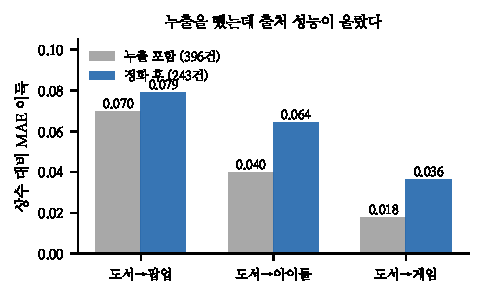
\includegraphics[width=\columnwidth]{figs/srcgain.pdf}
\caption{도서를 출처로 쓴 세 방향. 표본이 396에서 243으로 줄었는데 전부 좋아졌다.}
\end{figure}

표본을 39\% 버렸는데 도서를 출처로 쓴 세 방향이 \emph{모두} 좋아졌다. 누출이
정렬 기하를 오염시키고 있었다는 뜻이다.

\begin{figure}[t]
\centering
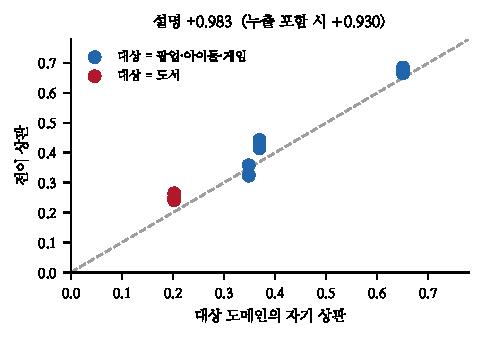
\includegraphics[width=\columnwidth]{figs/ceil2.pdf}
\caption{노트 33의 등식을 정화된 열두 셀에서 다시 잰 것.}
\end{figure}

\begin{table}[t]
\centering\tsize
\caption{노트 33 등식의 재확인.}
\begin{tabular}{lrr}
\toprule
& 누출 포함 & 정화 후 \\
\midrule
대상 자기 상관 설명 & $+$0.930 & \textbf{$+$0.983} \\
출처 자기 상관 설명 & $-$0.219 & $-$0.309 \\
비율 평균 & 0.936 & 1.098 \\
\bottomrule
\end{tabular}
\end{table}

노트 33의 등식이 더 깨끗해졌다. 노트 34가 한계로 적은 ``비율 평균 0.936이
1보다 작으니 출처 품질 하한이 있을 수 있다''도 해소된다 --- 그것은 누출 때문이었다.

\section{노트 34를 어디까지 정정하나}

\begin{itemize}[leftmargin=1.1em,itemsep=0.2em]
\item \textbf{유지} --- ``자기 상관은 도메인의 고정 성질이 아니라 배선의 함수다.''
      이 노트에서 도서 굿즈 규모를 바꿔 9/12를 유지하며 이득을 $+$0.0441에서
      $+$0.0473으로 올렸으니 오히려 재확인된다.
\item \textbf{철회} --- ``판형으로 배선하자 자기 상관이 0.100에서 0.344로
      3.4배.'' 그 상승분의 대부분은 판형이라는 물리량이 아니라 판형 결측이
      대리한 매체 형식이었다.
\item \textbf{철회} --- ``도서 라벨은 가용 피처 전부로 44.1\%가 설명되는
      압도적 1위.'' 그 44.1\%도 형식을 포함한 값이다.
\end{itemize}

\begin{quote}\fontsize{9.5}{11.5}\selectfont
배선으로 자기 상관을 올렸을 때 \textbf{무엇이 올랐는지 반드시 따로 확인해야
한다.} 올라간 것이 물리량인지, 표본 구성인지, 결측 패턴인지는 자기 상관 숫자만
보면 구분되지 않는다.
\end{quote}

\paragraph{도구가 자기를 만든 노트를 무너뜨렸다}
배선 탐색기는 노트 34의 결론을 실행하려고 만든 것이다. 그 도구의 첫 산출물이
노트 34의 사례를 철회시켰다. 이런 일이 반복되는 것이 이 루프가 작동하고 있다는
증거라고 본다.

\section{한계}

\begin{itemize}[leftmargin=1.1em,itemsep=0.15em]
\item 종이책 243건 안에도 무선(184)과 양장(57)이 섞여 있고 라벨 평균이 4.25 대
      4.47로 다르다. 같은 병의 약한 형태가 남아 있을 수 있다.
\item 전자책을 버린 것이지 다룬 것이 아니다. 전자책은 자기 상관 0.045로 축이
      전혀 설명하지 못하는데 그 이유를 보지 않았다.
\item 나머지 세 도메인에 같은 검사를 하지 않았다. 결측률이 높은 축은 아이돌의
      앨범 메타(85\%)와 게임의 하드웨어 요구(94\%)다.
\item 도서 비율이 1.19$\sim$1.31로 1을 크게 넘는다. 자기 상관 0.203이 n=243에서
      과소추정된 것일 수 있다.
\item 게임 폭$=$언어만은 자기 상관을 0.349에서 0.374로 올리는데 유의는 9/12로
      그대로다. 채택하지 않았고 이유도 모른다.
\end{itemize}

\section{다음}

\begin{enumerate}[leftmargin=1.3em,itemsep=0.15em]
\item 결측 패턴 누출을 네 도메인 전부에서 기계적으로 검사한다 --- 각 축의 마스크와
      라벨의 상관을 재는 것으로 충분하다.
\item 무선/양장 층화가 남긴 몫을 잰다.
\item 게임 폭$=$언어만이 자기 상관만 올리고 전이를 못 올리는 이유.
\item 전자책을 별도 도메인으로 세울 수 있는지 --- 축이 아예 다를 수 있다.
\end{enumerate}

\vspace{0.6em}
\hrule height 0.3pt
\vspace{0.5em}
{\footnotesize
\textbf{참고문헌}\\[0.3em]
Kaufman, S., Rosset, S., Perlich, C. (2012). Leakage in data mining:
formulation, detection, and avoidance. \emph{ACM TKDD}, 6(4), 1--21.\\[0.15em]
Rubin, D. B. (1976). Inference and missing data. \emph{Biometrika}, 63(3), 581--592.\\[0.15em]
Horst, P. (1941). The role of predictor variables which are independent of the
criterion. \emph{Social Science Research Council}, 48, 431--436.\\[0.15em]
Little, R. J. A., Rubin, D. B. (2019). \emph{Statistical Analysis with Missing
Data}, 3rd ed. Wiley.\\[0.15em]
Ben-David, S. et al. (2010). A theory of learning from different domains.
\emph{Machine Learning}, 79(1--2), 151--175.
}

\end{document}
